
\documentclass{article}
\usepackage{graphicx}
\usepackage{natbib}

\newcommand{\given}{\,|\,}

\bibliographystyle{sysbio}

\begin{document}



\begin{center}

{\Large\bf RevBayes}

\bigskip

{\sc Sebastian H\"ohna$^{1}$, John P. Huelsenbeck$^{2}$, Fredrik Ronquist$^{3}$} \\

\bigskip

{\em
$\mbox{}^1$Department of Mathematics, Stockholm University, Stockholm, Sweden \\

$\mbox{}^2$Department of Integrative Biology, University of California, Berkeley\\

$\mbox{}^3$Swedish Museum of Natural History, Stockholm, Sweden. \\

}
\end{center}

\bigskip

\noindent RevBayes is a program for the Bayesian estimation of phylogeny. 
The program takes as input character matrices, such as alignments of DNA or amino acid sequences.
RevBayes uses a numerical method called Markov chain Monte Carlo \citep[MCMC;][]{metropolis53,hastings70} to approximate
the posterior probabilities of phylogenetic trees; the program's output consists of files containing the MCMC samples. 
The MCMC samples can then be summarized in a variety of ways to make inferences about the phylogeny of the group of interest
as well as other parameters of the phylogenetic model.

RevBayes grew out of developments in the MrBayes program \citep{huelsenbeck01c,ronquist03}.
Although the MrBayes program was quite popular, F.R. and J.P.H. made design decisions when writing MrBayes that made it difficult
to accommodate new developments in the field. For example, MrBayes --- like all phylogenetic programs --- considers the phylogenetic
model to be fixed. However, new developments allow the phylogenetic model itself to be considered an object of 
inference \citep[{\it e.g.},][]{huelsenbeck04d}. Similarly, although MrBayes allows the user to partition data and model the evolutionary
process independently in each data subset, it does not allow the partitioning scheme itself to be an object of inference. Instead,
the user must specify the partition, which then remains an assumption of the analysis. New developments in the field, however, allow
the partition itself to be considered a parameter to be estimated \citep{lartillot04,huelsenbeck06,huelsenbeck07b} or allow the
evolution at an alignment site to be considered a mixture from several different models \citep{pagel04,pagel05}. 
Implementing these new developments would require extensive rewriting of the MrBayes code. 

One other limitation of the MrBayes program strongly guided the development of RevBayes: MrBayes uses a method for specifying
evolutionary models that is quite limited. MrBayes, in an exercise of M\"ullerian mimicry\footnote{M\"ullerian mimicry, for the 
unfamiliar reader, is a phenomenon where two species that are both distasteful to predators evolve the same warning coloration.
This is by contrast to Batesian mimicry, where a palatable species evolves a coloration similar to a distasteful species.
We thought it unkind to describe PAUP* as the exclusively distasteful species when using the mimicry metaphore; we therefore call
MrBayes a M\"ullerian mimic.}, 
uses a command line interface and
method for specifying models that closely resembles that used by PAUP* \citep{swofford98}, arguably the phylogeny program that has
been the most influential in the field.
However, we needed a language that was well-suited to specifying probability models which, after all, are what a Bayesian analysis assumes,
and that could be easily extended; the MrBayes model-specification method placed constraints on how easily complex models could be described.
Moreover, we wanted a language that could, in principle at least, allow the user to specify evolutionary
models that have never been considered before. 
After careful consideration of the limitations of the MrBayes design and language, 
the decision was made to discontinue development of MrBayes and completely rethink how a phylogenetic program --- specifically a
Bayesian phylogenetic program --- should be structured. The result is the RevBayes program.

This manual is intended to provide a background to the ideas implemented in the program and guidance on how to use the program.
RevBayes is a purely Bayesian program. This simplifies matters from the perspective of the RevBayes development team because
they do not need to consider ideas and methods that are not Bayesian. 
However, Bayesian statistical analysis can be quite complicated.
One goal of this manual is to supply the user the necessary background information on Bayesian analysis to perform an adept Bayesian
phylogenetic analysis.
Similarly, phylogenetic analysis has become an incredibly baroque field with an extensive literature. Another goal of
this manual is to provide the user background on phylogenetic models. Finally, RevBayes uses a new language for specifying 
phylogenetic models that is quite powerful and similar to the R language \citep{ihaka96}. 
(The program has switched models and now is a M\"ullerian mimic of R.)
This manual provides background information necessary to specify complex phylogenetic models using RevBayes.

\section*{Bayesian Inference}

Statistics is a set of methods for making inferences about the world in the face of uncertainty.
In general, the statistical approach considers the data as potentially variable and assumes a 
probability model to describe this variability. 
For example, on tossing a coin the uncertainty in the 
outcome can be described by the Bernoulli model in which the 
probability of observing a head is $\theta$ and the probability of observing a tail is $1 - \theta$ 
(where $0 \leq \theta \leq 1$). 
The Bernoulli model expresses the uncertainty of the outcome of a coin toss by a single parameter, $\theta$. 
One of the main goals of statistical inference is to assign values to parameters of a model based on observations,
a process called `estimation'. 
For coin tossing, the goal may be to estimate the value of $\theta$ (the 
parameter of the Bernoulli model) based on the results of tossing a coin repeatedly 
(the data)\footnote{Throughout this manual, we use the convention of denoting the observations as $X$ and the parameters using greek letters,
such as $\theta$.
We also use the convention of describing a conditional probability as $f(\cdot \given \cdot)$. Because all probability  functions
are described in this manner, there is the potential for confusion. However, it should be clear
from the context and the parameters of the function what its identity is and whether the
probability distribution is  discrete or continuous.}. 

There are many methods for estimating the parameters of a statistical model. Here, we will consider only two: 
the method of maximum likelihood, first described by the great population geneticist and statistician R.\ A.\ Fisher, and 
Bayesian estimation. Maximum likelihood calls the best estimate of a parameter that parameter value that maximizes the probability
of the observations. This estimate is called the `maximum likelihood estimate' (or `MLE').
The probability of observing the data is called the likelihood function:
$$
L(\mbox{Parameter}) = C \times \Pr(\mbox{Observations} \given \mbox{Parameter})
$$
where the constant $C$ is arbitrary, but allows both continuous and discrete probability distributions to be evaluated.

\begin{figure}[t]
\begin{center}
\frame{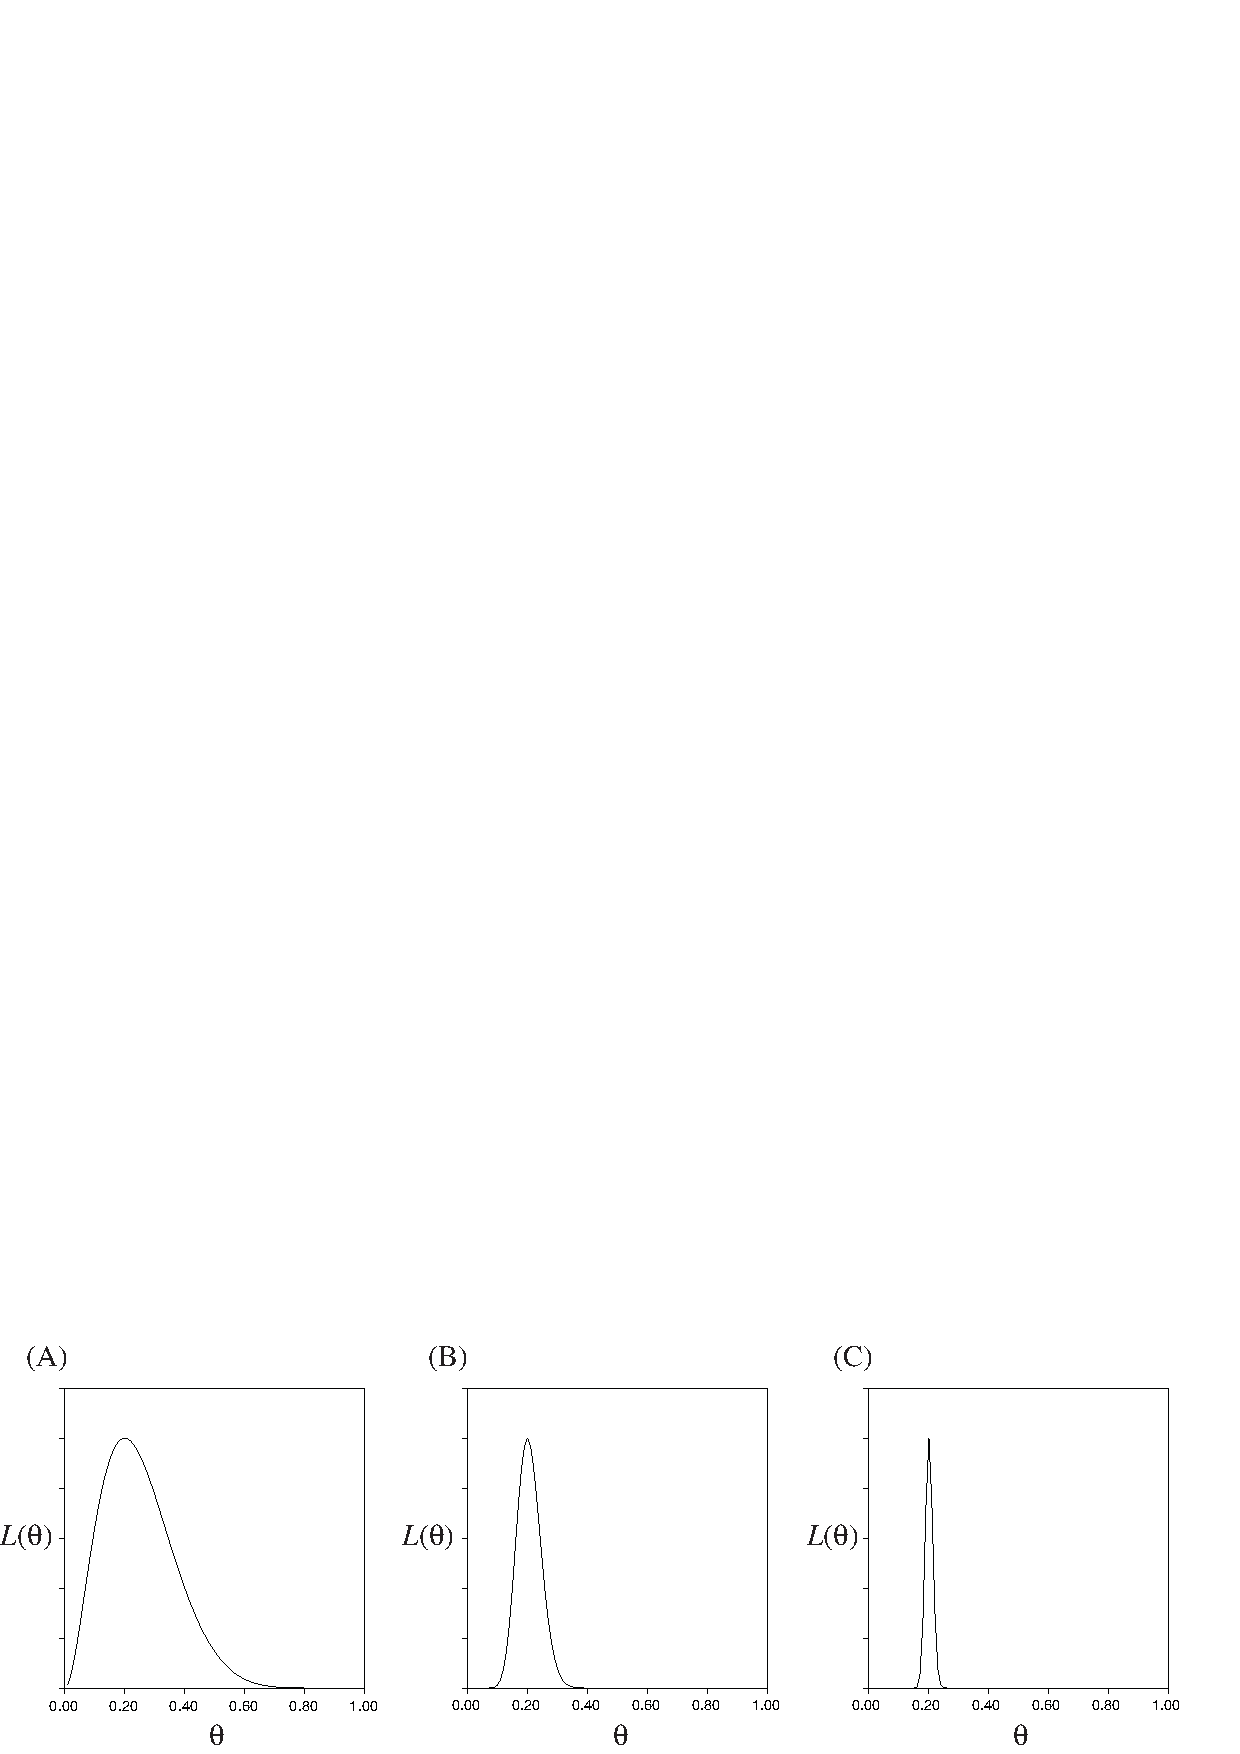
\includegraphics[width=4.75in]{figures/likelihood_coin}}
\end{center}
\caption{The likelihood function for three different sets of observations that all have the property of having the same
maximum likelihood estimate of $\hat{\theta} = 0.2$.
A, $n=10$ and $x=2$; B, $n=100$ and $x = 20$; C, $n=1000$ and $x = 200$.}
\label{coin_eg}
\medskip
\hrule
\end{figure}

A simple example illustrates the method of maximum likelihood. Consider the problem of estimating the probability that
heads appear face up on a single toss of a coin. For a fair coin, the probability that heads lands face-up on a single toss is $\theta = 1/2$.
However, one can also estimate the probability of heads for any particular coin; perhaps one is interested in testing whether 
the coin is, indeed, a fair one. In this case, the parameter $\theta$ is considered a parameter of the statistical model, and is
allowed to vary. As a scientist, the natural way to determine whether some coin is in fact fair is to toss the coin many times ({\it i.e.}, 
the scientist performs an experiment). One way to summarize the results of a coin-tossing experiment is to simply note the number of
times heads land face up on $n$ tosses of the coin. We will denote the number of heads observed on $n$ tosses $x$. The likelihood for the coin
tossing experiment is 
$$
L(\theta) = {n \choose x} \theta^x (1-\theta)^{n-x}
$$
which is the binomial probability distribution. (The binomial coefficient, ${n \choose x} = {n! \over x!(n-x)!}$, is the number of
ways to choose $x$ objects from $n$.)

Figure \ref{coin_eg} plots the parameter $\theta$ against the likelihood for several different experimental outcomes. Note that the likelihood appears
to be maximized when $\theta$ is equal to the proportion of heads that were observed. With a modest amount of
calculus, one can show that the likelihood is in fact maximized at $\theta = x/n$. 

\section*{Bayesian Inference of Phylogeny}

\section*{Phylogenetic Models}

\section*{Graphical Representation of Probability Models}

\section*{Acknowledgments}

Sebastian H\"ohna thanks his m\"utterchen.
The development of RevBayes was partially supported by grants from the NSF (DEB-0918791) and NIH ([NUMBER]) awarded to J.P.H.

\bibliography{../bayes}

\newpage


\end{document}
